%%%%%%%%%%%%%%%%%%%%%%%%%%%%%%%%%%%%%%%%%%%
%
% Document class
%
% Change this if you want a different size/orientation poster etc.
%
%%%%%%%%%%%%%%%%%%%%%%%%%%%%%%%%%%%%%%%%%%%

%\documentclass[landscape,a0b,final,a4resizeable]{a0poster}
%\documentclass[portrait,a0b,final,a4resizeable]{a0poster}
%\documentclass[portrait,a0b,final]{a0poster}
\documentclass[portrait,a0b,final]{a0poster}

\usepackage{etex}

%%%%%%%%%%%%%%%%%%%%%%%%%%%%%%%%%%%%%%%%%%%
%
% Basic packages
%
%%%%%%%%%%%%%%%%%%%%%%%%%%%%%%%%%%%%%%%%%%%

\usepackage{multicol}
\usepackage{color}
\usepackage{shadow}
\usepackage{morefloats}
\usepackage[pdftex]{graphicx}
\usepackage{rotating}
\usepackage{amsmath, amsthm, amssymb, amsfonts}
\usepackage{amsfonts,dsfont}
\usepackage{array}
\usepackage{nth}
\usepackage{booktabs}
\usepackage{bbm}
\usepackage{verbatim}

% To use the framed environment 
\usepackage{framed} 

% Bibliography without title.
\usepackage[square, numbers, comma]{natbib}
\renewcommand{\bibsection}{}

% Caption for use outside floats.
\newcommand{\myCaption}[1]{\parbox{\linewidth}{\large \vspace{10pt} #1 \vspace{10pt}}}

% Subfigures, etc.
\usepackage{subfigure}

%\usepackage{pagegrid}
\usepackage{eucal}

% My maths macros.
%\usepackage{mathsMacros}

% Orange emphasis.
\newcommand{\oEmph}[1]{\textcolor{orange}{#1}}

% My commands.
\newcommand{\Exponential}{\mathrm{Exp}}
\newcommand{\diff}{\mathrm{d}}
\newcommand{\grad}{\nabla}
\newcommand{\Ind}{\mathbb{I}}
\newcommand{\Uniform}{\mathrm{Uniform}}
\newcommand{\lambdaref}{\lambda_{\text{ref}}}

%%%%%%%%%%%%%%%%%%%%%%%%%%%%%%%%%%%%%%%%%%%
%
% TIKZ packages and common definitions
%
% Add extra things as per your tikz needs
%
%%%%%%%%%%%%%%%%%%%%%%%%%%%%%%%%%%%%%%%%%%%

\usepackage{picins}
\usepackage{tikz}
\usetikzlibrary{shapes.geometric,arrows,chains,matrix,positioning,scopes,calc}
\tikzstyle{mybox} = [draw=white, rectangle]

\graphicspath{{PosterFigures/}{PaperFigures/}{Branding/}}

%%%%%%%%%%%%%%%%%%%%%%%%%%%%%%%%%%%%%%%%%%%
%
% Some standard colours
%
%%%%%%%%%%%%%%%%%%%%%%%%%%%%%%%%%%%%%%%%%%%

\definecolor{oxdarkblue}{cmyk}{1, 0.8, 0, 0.6}
\definecolor{lightblue}{rgb}{0, 0, 0.80}
\definecolor{white}{rgb}{1, 1, 1}
\definecolor{whiteblue}{rgb}{0.80, 0.80, 1}

%%%%%%%%%%%%%%%%%%%%%%%%%%%%%%%%%%%%%%%%%%%
%
% Some look and feel definitions
%
%%%%%%%%%%%%%%%%%%%%%%%%%%%%%%%%%%%%%%%%%%%

\setlength{\columnsep}{0.05\textwidth}
\setlength{\columnseprule}{0.00025\textwidth}
\setlength{\parindent}{1cm}
\setlength{\parskip}{1cm}

%%%%%%%%%%%%%%%%%%%%%%%%%%%%%%%%%%%%%%%%%%%
%
% \mysection - replacement for \section*
% 
%%%%%%%%%%%%%%%%%%%%%%%%%%%%%%%%%%%%%%%%%%%

\tikzstyle{mysection} = [rectangle, 
	draw=none, 
	shade, 
	outer color=oxdarkblue,
	inner color=oxdarkblue,
	text width=0.97\columnwidth,
	text centered,
	text=white,
	rounded corners=20pt,
	minimum height=3cm]%0.11\columnwidth]

\newcommand{\mysection}[1]
{
	\begin{center}
		\begin{tikzpicture}
			\node[mysection] {\sffamily\bfseries\LARGE#1};
		\end{tikzpicture}
	\end{center}
}


\newcommand{\mysubsection}[1]
{
			{\sffamily\bfseries#1}
}


%%%%%%%%%%%%%%%%%%%%%%%%%%%%%%%%%%%%%%%%%%%%
%%
%% \myalign - replacement for {align*}
%% 
%%%%%%%%%%%%%%%%%%%%%%%%%%%%%%%%%%%%%%%%%%%%
%
%\tikzstyle{myalign} = [draw, rectangle, 
%	text width=\columnwidth,
%	text centered,
%	text=black]
%
%\newcommand{\myalign}[1]
%{
%	\begin{center}
%		\begin{tikzpicture}
%			\node[myalign] {\Large $ \begin{aligned} #1 \end{aligned} $};
%		\end{tikzpicture}
%	\end{center}
%}

%%%%%%%%%%%%%%%%%%%%%%%%%%%%%%%%%%%%%%%%%%%
%
% Set the font
%
%%%%%%%%%%%%%%%%%%%%%%%%%%%%%%%%%%%%%%%%%%%

\renewcommand{\familydefault}{cmss}
\sffamily

%%%%%%%%%%%%%%%%%%%%%%%%%%%%%%%%%%%%%%%%%%%
%
% New commands on theorem and proofs 
%
%%%%%%%%%%%%%%%%%%%%%%%%%%%%%%%%%%%%%%%%%%%
\newcommand{\iid}{\overset{i.i.d.}{\sim}}


%%%%%%%%%%%%%%%%%%%%%%%%%%%%%%%%%%%%%%%%%%%
%
% Poster environment
%
%%%%%%%%%%%%%%%%%%%%%%%%%%%%%%%%%%%%%%%%%%%

\newenvironment{poster}
{
	\begin{center}
		\hspace{-2in}
		\begin{minipage}[c]{0.96\textwidth}
		}
		{
		\end{minipage} 
	\end{center}
}

%%%%%%%%%%%%%%%%%%%%%%%%%%%%%%%%%%%%%%%%%%%
%
% The document environment starts here
%
%%%%%%%%%%%%%%%%%%%%%%%%%%%%%%%%%%%%%%%%%%%

\begin{document}

%%%%%%%%%%%%%%%%%%%%%%%%%%%%%%%%%%%%%%%%%%%
%
% Begin the poster environment - centres things etc
%
%%%%%%%%%%%%%%%%%%%%%%%%%%%%%%%%%%%%%%%%%%%

\begin{poster}

\vspace{1\baselineskip}

%%%%%%%%%%%%%%%%%%%%%%%%%%%%%%%%%%%%%%%%%%%
%
% Draw the header as a TIKZ picture
%
%%%%%%%%%%%%%%%%%%%%%%%%%%%%%%%%%%%%%%%%%%%

\nocite{vanetti2017piecewise}

\begin{center}
	\begin{tikzpicture}
		\begin{scope}

			\node[inner sep=0, text width=0.64\textwidth, text centered, anchor=north west, font=\Huge] (Title) at (0, 0) 
			{
				{\sffamily
                                  \Huge \textbf{Title} \\
                                } 
				{\sffamily\huge    Author}\\

                                {\LARGE \texttt{email@adress}}
			};


                        \node[mybox, anchor=north west] (box) at ($(Title.north east) + (0, 0 em) $)
                        {
                          
\includegraphics[width=0.32\textwidth]{Branding/Mathematics_2col_cmyk.eps}
                        };

                
		\end{scope}
	\end{tikzpicture}
\end{center}

%%%%%%%%%%%%%%%%%%%%%%%%%%%%%%%%%%%%%%%%%%%
%
% Spacing between title and main body
%
%%%%%%%%%%%%%%%%%%%%%%%%%%%%%%%%%%%%%%%%%%%

%\vspace{2\baselineskip}
%\vspace{1\baselineskip} % Add this back in!

%%%%%%%%%%%%%%%%%%%%%%%%%%%%%%%%%%%%%%%%%%%
%
% Main body
%
%%%%%%%%%%%%%%%%%%%%%%%%%%%%%%%%%%%%%%%%%%%

\Large % this gives the font size, for detail see: http://www.ctex.org/documents/packages/nonstd/a0poster.pdf


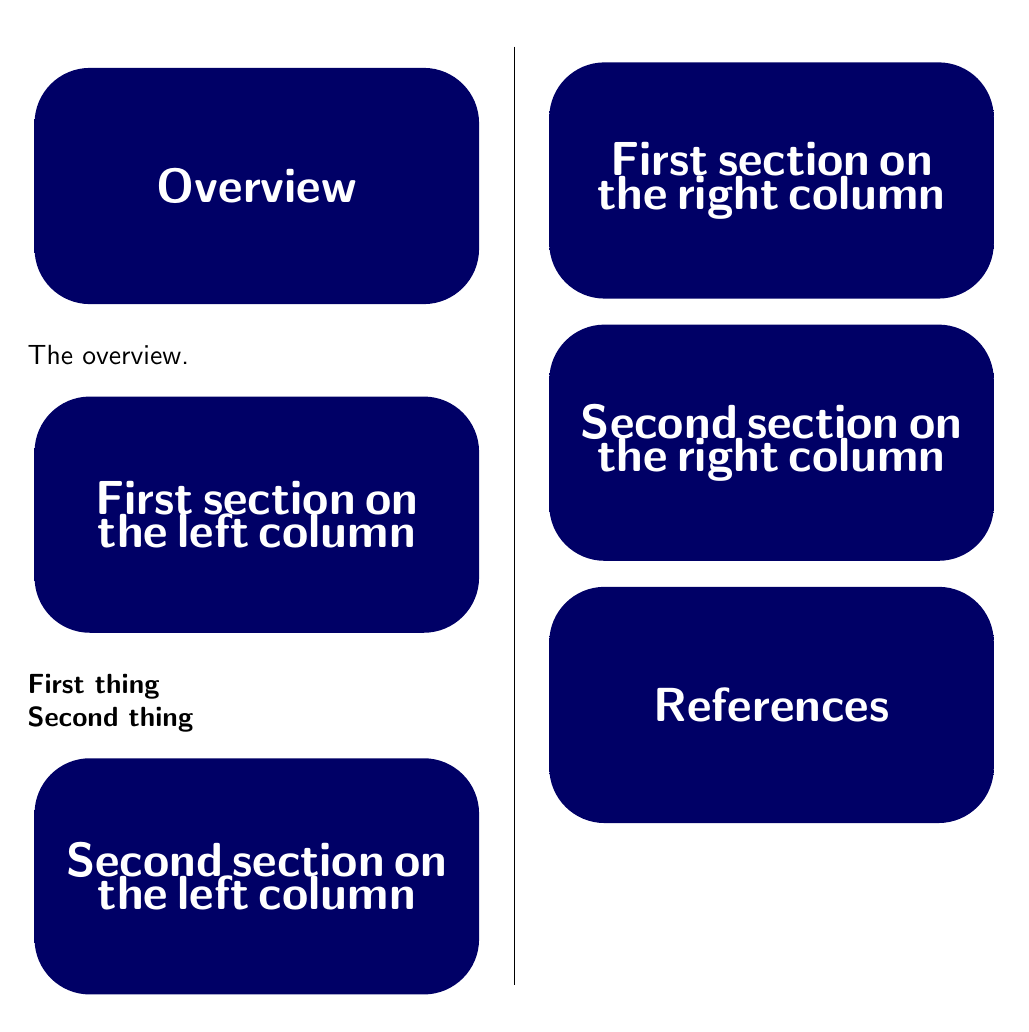
\begin{tikzpicture}
\begin{scope}

\node (n1) [text width=0.48\textwidth, align = justify, anchor = north west, inner sep = 0] at (3em, 0)
{

\mysection{Overview}

The overview.

};


\node (n1b) [text width=0.48\textwidth, align = justify, anchor = north west, inner sep = 0] at ($(n1.south west) + (0, 0) $)
{

\mysection{First section on the left column}

\textbf{First thing} 

\textbf{Second thing}


};






\node (n1c) [text width=0.48\textwidth, align = justify, anchor = north west, inner sep = 0] at ($ (n1b.south west) + (0, 0) $)
{
\mysection{Second section on the left column}


};


\node (n20) [text width=0.48\textwidth, align = justify, anchor = north west, inner sep = 0] at ($ (n1.north east) + (2em, 0) $)
{
	\mysection{First section on the right column}
	
	
};

\node (n21) [text width=0.48\textwidth, align = justify, anchor = north west, inner sep = 0] at ($(n20.south west) + (0, 0) $)
{
\mysection{Second section on the right column}



};


\node (n22) [text width=0.48\textwidth, align = justify, anchor = north west, inner sep = 0] at ($ (n21.south west)$)
{
\mysection{References}

{
%	You can include your bibliography in a bib file here
%\normalsize
%\bibliographystyle{apalike}
%\bibliography{ }

}

};

%%%%%%%%%%%%%%%%%%%%%%%%%%%%%%%%%%%%%%%%%%%
%
% Decorative lines.
%
%%%%%%%%%%%%%%%%%%%%%%%%%%%%%%%%%%%%%%%%%%%



% this is a separating line between  the two text columns
\node (l1) at ($ (n1.north east) + (1em, 0) $) {};
\node (l2) at ($ (n1c.south east) + (1em, 0) $) {};
\draw[black] (l1) -- (l2);


%\node (l3) at ($ (n7.north east) + (0.025\linewidth, 0) $) {};
%\node (l4) at ($ (l2) + (0.35\linewidth, 0) $) {};
%\draw[black] (l3) -- (l4);


\end{scope}
\end{tikzpicture}

\end{poster}

\end{document}
